\subsection{Perceptual Hashing}
Neben der mittleren quadratischen Abweichung ist eine der einfachsten, aber auch
anfälligsten Methoden zur Bestimmung der Ähnlichkeit von zwei Bildern das
Hashing. Dabei gibt es viele verschiedene Ansätze und Vorgehensmodelle. Die
gängigste Methode ist die Anwendung des pHashes, auch genannt Perceptual Hashing.
\parencite{hashing-apiumhub}

Beim Perceptual Hashing werden sowohl für Bild A als auch für Bild B ein Hash
berechnet. Die daraus resultierende Hamming-Distanz zwischen den Hashes ergibt
die Ähnlichkeit der Bilder. Je geringer die Distanz, desto ähnlicher. Das
Verfahren ist nicht normiert und noch ein offenes
Forschungsthema. \parencite{hashing-phash}

Im Folgenden wird ein beispielhaftes pHash-Verfahren erläutert. Zuerst wird
sowohl das Referenz- als auch das Suchbild in eine Graustufen-Grafik
umgewandelt. Schließlich wird die Grafik auf 32x32 Pixel skaliert. Auf das
entstandene Grauwertbild folgen zwei Diskrete Kosinus Transformationen (1. Pro
Zeile, 2. Pro Spalte). Die hochfrequenten Abschnitte befinden sich nun links
oben in einer 8x8 Matrix. Daraufhin wird der Median-Grauwert der 64 Pixel
berechnet. Jeder Pixel, dessen Grauwert unter dem Durchschnitt liegt wird weiß
eingefärbt, der Rest schwarz. Daraus ergibt sich ein 64-Bit langer Hashwert
(schwarz: 0, weiß: 1). Zuletzt wird durch eine Subtraktion der beiden
generierten Bitfolgen die Hamming-Distanz berechnet. Mittels einem vorher
festgelegten Schwellenwert wird jetzt auf Basis des Hamming-Abstands bestimmt,
ob die Bilder als ähnlich eingestuft werden. Je niedriger der Abstand, desto
größer die Übereinstimmung. \parencite{hashing-apiumhub}

\noindent{\textbf{Vorteile}}
\begin{itemize}[topsep=0pt]
    \item Schnelle Suchperformance, wenn die Hashes der Referenzbilder bereits
    in einer dafür geeigneten Datenstruktur (z.B. k-d-Bäume, VP Bäume oder
    Kugelbäume) vorliegen \parencite{hashing-lvngd}
    \item Einfach zu implementieren
    \item Robust gegen Wasserzeichen, Farbfilter, leichte Helligkeits- und
    Kontraständerungen, Gammakorrekturen, Skalierungen sowie Komprimierungen
    (siehe Abbildung \ref{fig:phash})
    \parencite{hashing-phash}
\end{itemize}

\noindent{\textbf{Nachteile}}
\begin{itemize}[topsep=0pt]
    \item Nicht robust gegen Spiegelungen, Rotierungen und Verzerrungen (siehe
    Abbildung \ref{fig:phash}))
    \item Nicht robust gegen Zuschneidungen, neu eingefügten Elementen oder
    Änderungen des Blickwinkels
\end{itemize}

\begin{figure}[H]
    \centering
    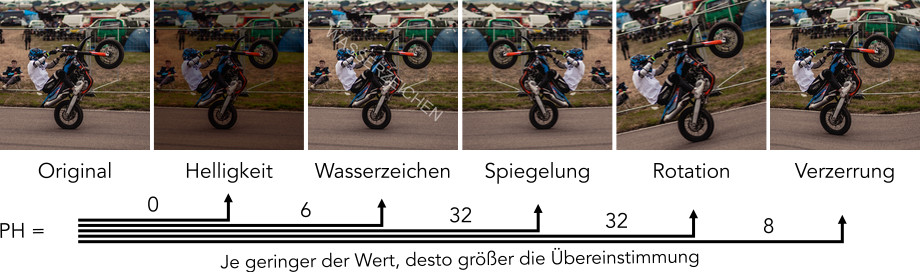
\includegraphics[width=\textwidth]{phash}
    \caption{PHASH: Anwendung an verschiedenen Testbildern}
    \label{fig:phash}
    \bildquelle{Eigene Darstellung}
\end{figure}